\begin{frame}[fragile]{Schema del database World}
\begin{figure}
    \centering
        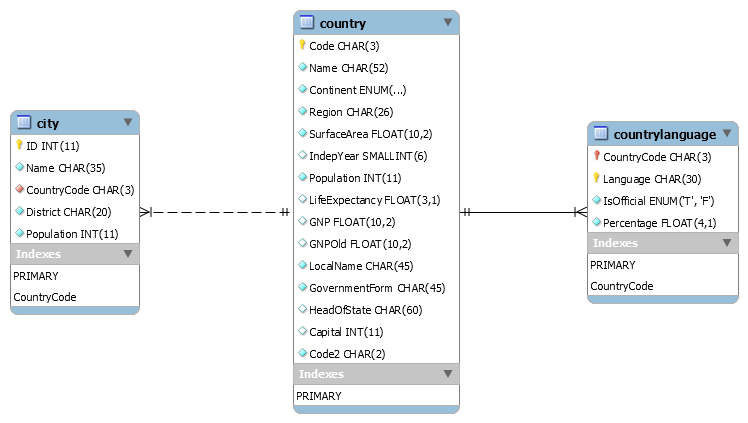
\includegraphics[width=.8\textwidth]{img/db-world.png}
    \end{figure}
\end{frame}
%
\begin{frame}[fragile]{World: Es. 1}
Visualizzare id, nome, popolazione dalla tabella \textit{city} e limitare i risultati solo alle prime 10 righe.
\pause
\begin{lstlisting}
SELECT Id, Name, Population
FROM city
LIMIT 10;
\end{lstlisting}
\end{frame}
%
\begin{frame}[fragile]{World: Es. 2}
Visualizzare id, nome, popolazione dalla tabella \textit{city} e limitare i risultati alle righe 31-40.
\pause
\begin{lstlisting}
SELECT Id, Name, Population
FROM city
LIMIT 30, 10;
\end{lstlisting}
\end{frame}
%
\begin{frame}[fragile]{World: Es. 3}
Trovare dalla tabella \textit{city} solo le citt\`a la cui popolazione \`e superiore a 2000000.
\pause
\begin{lstlisting}
SELECT Name, Population
FROM city
WHERE Population > 2000000;
\end{lstlisting}
\end{frame}
%
\begin{frame}[fragile]{World: Es. 4}
Trovare tutti i nomi di citt\`a dalla tabella \textit{city} il cui nome inizia con il prefisso ``Be''.
\pause
\begin{lstlisting}
SELECT Name
FROM city
WHERE Name LIKE `Be%';
\end{lstlisting}
\end{frame}
%
\begin{frame}[fragile]{World: Es. 5}
Trovare dalla tabella \textit{city} solo le citt\`a la cui popolazione \`e compresa tra 500000 e 1000000.
\pause
\begin{lstlisting}
SELECT Name, Population
FROM city
WHERE Population BETWEEN 500000 AND 1000000;
\end{lstlisting}
\pause
oppure
\begin{lstlisting}
SELECT Name, Population
FROM city
WHERE Population >= 500000 AND Population <=1000000;
\end{lstlisting}
\end{frame}
%
\begin{frame}[fragile]{World: Es. 6}
Visualizzare tutte le citt\`a della tabella \textit{city} ordinate per nome in ordine crescente.
\pause
\begin{lstlisting}
SELECT *
FROM city
ORDER BY Name ASC;
\end{lstlisting}
oppure
\pause
\begin{lstlisting}
SELECT *
FROM city
ORDER BY Name;
\end{lstlisting}
\end{frame}
%
\begin{frame}[fragile]{World: Es. 7}
Trovare la citt\`a con la popolazione pi\`u bassa nella tabella \textit{city}.
\pause
\vspace{-.1cm}
\begin{lstlisting}
SELECT Population, Name
FROM city
WHERE Population IS NOT NULL
ORDER BY Population ASC
LIMIT 1;
\end{lstlisting}
\end{frame}
%
\begin{frame}[fragile]{World: Es. 7}
Trovare la citt\`a con la popolazione pi\`u bassa nella tabella \textit{city}.

Altra possibile soluzione:
\vspace{-.1cm}
\begin{lstlisting}
SELECT MIN(Population), Name
FROM city
GROUP BY Name,Population
HAVING MIN(Population) ORDER BY Population
LIMIT 1;
\end{lstlisting}
\end{frame}
%
\begin{frame}[fragile]{World: Es. 8}
Trovare la citt\`a con la popolazione pi\`u bassa nella tabella \textit{city}.
\\Altra possibile soluzione:
\pause
\\Prima troviamo la \textbf{popolazione pi\`u bassa}:
\begin{lstlisting}
SELECT MIN(Population)
FROM country;
\end{lstlisting}
\pause
Poi facciamo una \textbf{query annidata} dove cerchiamo tutte le citt\`a che hanno poplazione = a quella appena trovata:
\begin{lstlisting}
SELECT Name, Population
FROM country
WHERE Population = (
    SELECT MIN(Population)
    FROM country
);
\end{lstlisting}
\end{frame}
%
\begin{frame}[fragile]{World: Es. 9}
Trovare il paese con la popolazione pi\`u numerosa nella tabella \textit{country}.
\pause
\begin{lstlisting}
SELECT Population, Name
FROM country
WHERE Population IS NOT NULL
ORDER BY Population DESC
LIMIT 1;
\end{lstlisting}
\end{frame}
%
\begin{frame}[fragile]{World: Es. 9}
Trovare il paese con la popolazione pi\`u numerosa nella tabella \textit{country}.

Altra soluzione possibile:
\pause
\\Prima troviamo la \textbf{pi\`u alta aspettativa di vita}:
\begin{lstlisting}
SELECT MAX(Population)
FROM country;
\end{lstlisting}
\pause
Poi facciamo una \textbf{query annidata} dove cerchiamo tutte le citt\`a che hanno come popolazione quella appena trovata:
\begin{lstlisting}
SELECT Population, Name
FROM country
WHERE Population = (
    SELECT MAX(Population)
    FROM country
);
\end{lstlisting}
\end{frame}
%
\begin{frame}[fragile]{World: Es. 10}
Elencare tutte le lingue parlate nella regione dei Caraibi (``Caribbean''). 
\pause
\begin{lstlisting}
SELECT country.Region, countrylanguage.Language
FROM country LEFT JOIN countrylanguage
ON country.Code = countrylanguage.CountryCode
WHERE country.Region = ``Caribbean'';
\end{lstlisting}
\end{frame}
%
\begin{frame}[fragile]{World: Es. 11}
Trovare la capitale della Spagna (ESP).
\pause
\begin{lstlisting}
SELECT city.Name
FROM city JOIN country ON city.ID = country.Capital
WHERE city.CountryCode = 'ESP';
\end{lstlisting}
\end{frame}
%
\begin{frame}[fragile]{World: Es. 12}
Trovare il paese con la pi\`u alta aspettativa di vita.
\pause
\begin{lstlisting}
SELECT country.Name, LifeExpectancy
FROM country
ORDER BY LifeExpectancy DESC
LIMIT 1;
\end{lstlisting}
\end{frame}
%
\begin{frame}[fragile]{World: Es. 12}
Trovare il paese con la pi\`u alta aspettativa di vita.

Altra soluzione Possibile:
\pause
\\Prima troviamo la \textbf{pi\`u alta aspettativa di vita}:
\begin{lstlisting}
SELECT MAX(LifeExpectancy)
FROM country;
\end{lstlisting}
\pause
Poi facciamo una \textbf{query annidata} dove cerchiamo quell'aspettativa di vita appena trovata:
\begin{lstlisting}
SELECT country.Name, LifeExpectancy
FROM country
WHERE LifeExpectancy = (
    SELECT MAX(LifeExpectancy)
    FROM country
);
\end{lstlisting}
\end{frame}
%
\begin{frame}[fragile]{World: Es. 13}
Trovare tutte le citt\`a del continente europeo.
\pause
\begin{lstlisting}
SELECT city.Name
FROM city JOIN country ON city.CountryCode = country.Code
WHERE country.Continent = 'Europe';
\end{lstlisting}
\end{frame}
%
\begin{frame}[fragile]{World: Es. 14}
Aggiornare il presidente degli Stati Uniti attualmente presente sul database, con `Donald Trump'.
\pause
\begin{lstlisting}
UPDATE country
SET HeadOfState = `Donald Trump'
WHERE Name = `United States';
\end{lstlisting}
\end{frame}
%
\begin{frame}[fragile]{World: Es. 15}
Trovare la citt\`a pi\`u popolata nella tabella \textit{city}.
\pause
\newline
\\Stesso ragionamento delle query precedenti (query annidata):
\begin{lstlisting}
SELECT Name, Population
FROM city
WHERE Population = (
    SELECT MAX(Population)
    FROM city
);
\end{lstlisting}
\end{frame}
%
\begin{frame}[fragile]{World: Es. 16}
Trovare la citt\`a meno popolata nella tabella \textit{city}.
\pause
\newline
\\Stesso ragionamento delle query precedenti (query annidata):
\begin{lstlisting}
SELECT Name, Population
FROM city
WHERE Population = (
    SELECT MIN(Population)
    FROM city
);
\end{lstlisting}
\end{frame}
%
\begin{frame}[fragile]{World: Es. 17}
Calcolare il numero di record della tabella \textit{city}.
\pause
\begin{lstlisting}
SELECT COUNT(Id) AS `n. di citta'
FROM city;
\end{lstlisting}
\end{frame}
%
\begin{frame}[fragile]{World: Es. 18}
Ottenere il numero di citt\`a in Cina dalla tabella \textit{city}.

La Cina ha country code ``CHN''.
\pause
\begin{lstlisting}
SELECT COUNT(*)
FROM city
WHERE CountryCode = ``CHN'';
\end{lstlisting}
\end{frame}
%